% Options for packages loaded elsewhere
\PassOptionsToPackage{unicode}{hyperref}
\PassOptionsToPackage{hyphens}{url}
\documentclass[
]{article}
\usepackage{xcolor}
\usepackage{amsmath,amssymb}
\setcounter{secnumdepth}{-\maxdimen} % remove section numbering
\usepackage{iftex}
\ifPDFTeX
  \usepackage[T1]{fontenc}
  \usepackage[utf8]{inputenc}
  \usepackage{textcomp} % provide euro and other symbols
\else % if luatex or xetex
  \usepackage{unicode-math} % this also loads fontspec
  \defaultfontfeatures{Scale=MatchLowercase}
  \defaultfontfeatures[\rmfamily]{Ligatures=TeX,Scale=1}
\fi
\usepackage{lmodern}
\ifPDFTeX\else
  % xetex/luatex font selection
\fi
% Use upquote if available, for straight quotes in verbatim environments
\IfFileExists{upquote.sty}{\usepackage{upquote}}{}
\IfFileExists{microtype.sty}{% use microtype if available
  \usepackage[]{microtype}
  \UseMicrotypeSet[protrusion]{basicmath} % disable protrusion for tt fonts
}{}
\makeatletter
\@ifundefined{KOMAClassName}{% if non-KOMA class
  \IfFileExists{parskip.sty}{%
    \usepackage{parskip}
  }{% else
    \setlength{\parindent}{0pt}
    \setlength{\parskip}{6pt plus 2pt minus 1pt}}
}{% if KOMA class
  \KOMAoptions{parskip=half}}
\makeatother
\usepackage{graphicx}
\makeatletter
\newsavebox\pandoc@box
\newcommand*\pandocbounded[1]{% scales image to fit in text height/width
  \sbox\pandoc@box{#1}%
  \Gscale@div\@tempa{\textheight}{\dimexpr\ht\pandoc@box+\dp\pandoc@box\relax}%
  \Gscale@div\@tempb{\linewidth}{\wd\pandoc@box}%
  \ifdim\@tempb\p@<\@tempa\p@\let\@tempa\@tempb\fi% select the smaller of both
  \ifdim\@tempa\p@<\p@\scalebox{\@tempa}{\usebox\pandoc@box}%
  \else\usebox{\pandoc@box}%
  \fi%
}
% Set default figure placement to htbp
\def\fps@figure{htbp}
\makeatother
\setlength{\emergencystretch}{3em} % prevent overfull lines
\providecommand{\tightlist}{%
  \setlength{\itemsep}{0pt}\setlength{\parskip}{0pt}}
\usepackage{bookmark}
\IfFileExists{xurl.sty}{\usepackage{xurl}}{} % add URL line breaks if available
\urlstyle{same}
\hypersetup{
  hidelinks,
  pdfcreator={LaTeX via pandoc}}

\author{}
\date{}

\begin{document}

{
\setcounter{tocdepth}{3}
\tableofcontents
}
Paul Koop

Das Pompeji-Projekt

Die letzte Freiheit

Kein System ist unfehlbar.

Es gibt immer eine Lücke.

Eine Erzählung aus dem Pompeji-Projekt

\emph{Überwachung, Widerstand und die Suche nach einem Ort, an dem Algorithmen nicht entscheiden.}

Inhaltsverzeichnis

\hyperref[annas-leben-in-der-encryption-and-telecommunication-zone]{\textbf{Annas Leben in der Encryption and Telecommunication Zone 2}}

\hyperref[anna-lernt-leonard-kennen]{\textbf{Anna lernt Leonard kennen 6}}

\hyperref[der-abend-in-der-stadt]{\textbf{Der Abend in der Stadt 10}}

\hyperref[die-entdeckung-von-ars]{\textbf{Die Entdeckung von ARS 13}}

\hyperref[geschichtsforschung-mit-ars]{\textbf{Geschichtsforschung mit ARS 22}}

\hyperref[die-ausreise]{\textbf{Die Ausreise 25}}

\hyperref[das-fluxfcchtlingslager]{\textbf{Das Flüchtlingslager 30}}

\hyperref[ein-neues-leben]{\textbf{Ein neues Leben 33}}

\hyperref[epilog]{\textbf{Epilog 36}}

\hyperref[einfluxfcsse-und-inspirationen-fuxfcr-das-pompeji-projekt-i.r.a.r.a.h]{\textbf{Einflüsse und Inspirationen für Das Pompeji-Projekt I.R.A.R.A.H 38}}

\section{Annas Leben in der Encryption and Telecommunication Zone}\label{annas-leben-in-der-encryption-and-telecommunication-zone}

Die Lichtstreifen der Überwachungskameras huschten über die kargen Betonwände des Quantencomputing ETZ, als Anna Jensen mit gesenktem Kopf durch die Sicherheitsschleuse trat. Das Summen der Scanner und das metallische Klicken der Zugangskarten waren ein ständiger Teil ihres Morgens. Sie wusste, dass jede Bewegung registriert wurde, jedes Muster ihres täglichen Weges durch die sterilen Korridore aufgezeichnet war -- eine Routine, die ihr längst zur Gewohnheit geworden war und doch wie ein unsichtbares Netz um sie lag.

Ihr Arbeitsplatz war eine Glaskabine, abgeschottet und doch durchsichtiger, als ihr lieb war. Auf dem Schreibtisch leuchteten die Bildschirme mit einer Kaskade von Datenströmen, die in grün-blauem Flimmern über die Anzeige jagten. Anna setzte sich, nahm die Kopfhörer ab, die sie gegen die monotone Geräuschkulisse der Serverräume abgeschirmt hatten, und schob eine lose Haarsträhne hinters Ohr. Für einen Moment verharrte sie, starrte auf die Zahlenreihen vor sich, die sich beständig veränderten.

Ihre Aufgabe bestand darin, Algorithmen zu optimieren, die verschlüsselte Kommunikationskanäle überwachten und Anomalien in den Datenströmen erkannten. Mit einem Tastendruck öffnete sie das Protokoll des Nachtdienstes. *Verdächtige Abweichungen: zwei.* Es war Routinearbeit. Doch je mehr Anna sich in die verschlüsselten Netzwerke vertiefte, desto stärker drängte sich ihr der Gedanke auf, dass sie in Wirklichkeit keinen Schutz für die Menschen erschuf -- sondern das perfekte Überwachungsinstrument.

Sie blinzelte und lehnte sich zurück, die Hände ruhten auf der Tastatur. Für einen Moment ließ sie den Blick über den Raum schweifen, als könnte sie dort eine Antwort finden. Aber alles, was sie sah, waren ihre eigenen Spiegelbilder in den Glaswänden und die gesichtslosen Silhouetten der anderen Mitarbeiter, die in ihren Kabinen über ihren Bildschirmen hingen. Die Luft war erfüllt vom gleichmäßigen Brummen der Server, einer Mischung aus mechanischer Präzision und menschlicher Gleichgültigkeit.

An diesem Morgen spürte Anna die Unruhe deutlicher als sonst -- ein leises, nagendes Gefühl im Bauch, das sich nicht abschütteln ließ. Die Vorstellung, dass jeder verschlüsselte Datenstrom, den sie prüfte, ein Leben war, das sich unbemerkt durch die Ritzen des Systems schlängeln wollte, ließ sie nicht los. Mit einem leichten Kopfschütteln rief sie sich selbst zur Ordnung, beugte sich wieder über die Tastatur. Doch in ihrem Hinterkopf nagte ein Gedanke: *Bin ich hier, um Menschen zu schützen -- oder nur, um ihre Freiheit weiter einzuschränken?*

Anna war sich nicht sicher, wann genau sie begonnen hatte, die ersten Zweifel zu hegen. Vielleicht war es das letzte Update gewesen, bei dem die Anweisungen plötzlich strenger, die Protokolle detaillierter geworden waren. Vielleicht der Gedanke, dass ihre Arbeit nicht mehr nur einem abstrakten Zweck diente, sondern in die intime Sphäre jeder Kommunikation eindrang. Oder war es etwas Tieferes, eine Sehnsucht nach einer Welt, die nicht durch die kalte Logik der Algorithmen beherrscht wurde?

Die Bildschirme flackerten weiter. Aber Anna konnte den Gedanken nicht abschütteln, dass sie Teil eines riesigen Apparates war, der die Menschen in unsichtbare Ketten legte.

Sie dachte an Leonard.

Er war vor einigen Wochen ins Team gekommen, aber seine ruhige, fast beiläufige Art, die Dinge in Frage zu stellen, war ihr sofort aufgefallen. In den kurzen Gesprächen in der Kaffeeküche hatte er einmal leise gesagt: „Manchmal frage ich mich, ob wir wirklich die Welt verbessern oder sie nur weiter einschränken.`` Sie hatte damals nicht geantwortet -- aber die Worte waren geblieben.

Ihr Blick wanderte zu seinem Schreibtisch. Er saß über seine Monitore gebeugt, die Stirn in Falten gelegt.

*Was wäre, wenn ich ihm meine Zweifel anvertraute?* Der Gedanke war verlockend -- und beängstigend zugleich. Leonard wirkte vertrauenswürdig, aber in diesem System konnte man sich nie sicher sein.

„Anna, alles in Ordnung?{\kern0pt}`` Die Stimme von Markus, einem Kollegen, riss sie aus ihren Gedanken. Er stand an der Tür ihrer Kabine, sein Gesicht hinter dem Glas leicht verzerrt, aber sie konnte die Besorgnis in seinen Augen erkennen.

„Ja, ich \ldots{} nur etwas nachdenklich``, antwortete sie und versuchte zu lächeln. Markus nickte verständnisvoll.

„Kommst du zur Besprechung? Ich glaube, sie wollen uns die neuesten Überwachungsprotokolle vorstellen``, sagte er.

„Natürlich, ich komme gleich``, murmelte Anna. Ihr Magen zog sich zusammen.

Die Versammlung fand in einem großen, anonymen Raum statt, dessen Wände mit Bildschirmen gefüllt waren, die ständig wechselnde Datenströme zeigten. Die Luft war elektrisch geladen. Anna setzte sich an einen der Tische, umgeben von Kollegen, deren Gesichter ausdruckslos blieben.

Herr Keller, ein älterer Mann mit einer Vorliebe für strenge Anzüge, betrat den Raum. „Willkommen zur heutigen Sitzung``, begann er mit einer Stimme, die so kalt war wie die Technik, die sie bedienten. „Wir stehen vor neuen Herausforderungen. Es ist unerlässlich, dass wir unsere Überwachungsmechanismen weiter optimieren, um die Stabilität der Autonomen Cities zu gewährleisten.``

Seine Worte hallten in Anna wider wie ein Echo der Unterdrückung. Sie spürte, wie Enttäuschung und Wut in ihr aufstiegen, während Herr Keller über die Notwendigkeit sprach, alle potenziellen Bedrohungen für das System zu eliminieren. Jedes Wort war ein Schlag ins Gesicht der Freiheit.

Während er die neuesten Algorithmus-Updates vorstellte, dachte Anna an die Menschen außerhalb dieser Wände. Familien, die sich nicht mehr frei bewegen konnten. Freunde, die nicht mehr offen miteinander sprechen durften. Mit einem Mal wurde ihr klar, dass sie nicht länger schweigen konnte.

Sie fühlte sich wie eine Fremde in ihrem eigenen Leben. Als die Sitzung endete, sammelte sie entschlossen ihre Sachen.

„Ich kann nicht mehr``, murmelte sie leise.

Die Mittagspause rückte näher. Anna spürte ein Kribbeln, als sie ihren Blick immer wieder zu Leonard wandern ließ. Als die Uhr die Pause ankündigte, schloss sie hastig ihr Protokoll. Leonard hatte sich erhoben und war auf dem Weg zur Cafeteria. Sie folgte ihm.

In der Cafeteria fanden sie eine ruhige Ecke.

„Wie läuft's bei dir?{\kern0pt}`` fragte Leonard.

„Ach, wie immer. Zahlen, Daten, Algorithmen``, antwortete sie mit einem schwachen Lächeln.

Leonard zuckte mit den Schultern. „Das Übliche. Manchmal frage ich mich, ob wir wirklich das Richtige tun.``

„Ich habe ähnliche Gedanken``, sagte Anna. „Ob es wirklich um Sicherheit geht oder um Kontrolle.``

Leonards Blick wurde intensiver. „Ich denke, es ist beides. Aber was zählt, ist, wie wir damit umgehen.``

Sie sprachen weiter -- über die ethischen Fragen ihrer Arbeit, über ihre Träume und Ängste. Es war ein Gespräch voller Offenheit.

Nach dem Mittagessen, in der Kaffeeküche, schlug Leonard vor: „Vielleicht könnten wir heute Abend zusammen essen?{\kern0pt}``

„Das klingt gut``, antwortete Anna, während ihr Herz schneller schlug.

Später, bei Leonard zu Hause, umgeben von einer warmen Atmosphäre und dem Duft von frischem Essen, schien die Zeit stillzustehen. Sie lachten, flirteten und öffneten sich einander.

„Es ist komisch, oder?{\kern0pt}``, sagte Anna mit einem schüchternen Lächeln. „Wie schnell wir hier gelandet sind.``

Leonard nickte, seine Augen funkelten. „Manchmal sind die besten Verbindungen die, die wir nicht planen.``

In diesem Moment schien alles möglich. Anna fühlte sich lebendig, als hätte sie einen Teil von sich selbst wiederentdeckt, den sie in den kühlen, sterilen Korridoren des ETZ verloren glaubte.

\section{Anna lernt Leonard kennen}\label{anna-lernt-leonard-kennen}

Die Tage nach ihrem Abendessen schienen von einer besonderen Spannung durchzogen zu sein, die Anna in jeder Begegnung mit Leonard spürte. Ihre Gespräche, die zunächst nur beiläufig und professionell wirkten, gewannen eine Tiefe, die sie überraschte. Es war, als hätte sich ein unsichtbarer Faden zwischen ihnen gespannt, der sie bei jeder Unterhaltung ein Stück näher zueinander zog.

Eines Nachmittags saßen sie in Annas Glaskabine. Die Bildschirme flimmerten mit den Datenströmen vor ihnen. Die Geräusche der Serverräume waren wie das Summen einer fernen Welt, das in der Stille ihrer Zusammenarbeit kaum noch von Bedeutung war.

„Es gibt immer mehr dieser kleinen Abweichungen``, murmelte Anna, während sie die Datenpakete analysierte. „Fast so, als würde jemand absichtlich versuchen, die Überwachungssysteme zu umgehen.``

Leonard beugte sich näher, sein Blick folgte den Zahlenreihen. „Vielleicht gibt es tatsächlich jemanden, der nach Schlupflöchern sucht. Oder es ist einfach ein Fehler im Algorithmus -- so perfekt, wie sie behaupten, ist die KI nicht.``

Anna hörte eine subtile Betonung in seiner Stimme. „Du glaubst also nicht, dass die Überwachung allmächtig ist?{\kern0pt}``

„Kein System ist unfehlbar``, antwortete Leonard, seine Augen blieben auf den Bildschirm gerichtet. „Es gibt immer eine Lücke. Man muss nur wissen, wie man sie findet.``

Anna nickte langsam. Ein Gedanke begann in ihr zu keimen -- faszinierend und beängstigend zugleich. „Was, wenn wir eine eigene Lücke schaffen könnten?{\kern0pt}`` fragte sie leise, als ob sie befürchtete, dass die Wände selbst lauschen könnten. „Einen Kommunikationskanal, der den Überwachungsalgorithmen entgeht?{\kern0pt}``

Leonard drehte sich zu ihr um. Sein Lächeln war herausfordernd und ermutigend zugleich. „Quantenverschlüsselung``, sagte er fast flüsternd. „Die Quantencomputer des ETZ sind mächtig genug, um solche Nachrichten zu dekodieren. Aber wenn wir die richtige Methode finden, könnte es gelingen, einen Kanal aufzubauen, der unbemerkt bleibt.``

Eine Welle der Aufregung durchströmte Anna. Die Möglichkeit, ein Kommunikationsnetzwerk zu schaffen, das sich der Kontrolle entzog, war mehr als eine technische Herausforderung -- es war ein Zeichen von Hoffnung. „Wir könnten das als Experiment tarnen``, schlug sie vor, ihre Stimme nun selbstbewusster. „Ein Forschungsprojekt zur Verbesserung der Sicherheitsprotokolle. Offiziell jedenfalls.``

Leonard nickte, seine Augen funkelten vor Begeisterung. „Und inoffiziell schaffen wir eine Möglichkeit, unabhängig zu kommunizieren.``

Die Idee begann Gestalt anzunehmen. Sie dachten über Details nach, entwarfen Algorithmen, analysierten Sicherheitslücken. Jedes Gespräch, jeder gemeinsam verbrachte Moment brachte sie näher aneinander -- aber auch näher an die gefährliche Realität, dass sie etwas erschaffen wollten, das über die Regeln hinausging.

Es war ein riskanter Plan. Aber für Anna fühlte es sich plötzlich lebendiger an als alles, was sie je getan hatte. Ihre Blicke begegneten sich immer häufiger. Die Nähe zwischen ihnen war nicht nur auf ihre gemeinsame Arbeit zurückzuführen. Es war ein unausgesprochener Bund aus Neugier und leiser Rebellion.

In den folgenden Tagen arbeiteten sie oft spät. Während der Rest des ETZ allmählich zur Ruhe kam, saßen sie in den stillen Stunden der Nacht über ihre Pläne gebeugt, die Gesichter von den Bildschirmen beleuchtet. Ihre Finger huschten in der Dunkelheit über die Tastaturen. Manchmal berührten sich ihre Hände -- kleine, bedeutungsvolle Berührungen, die ein Gefühl von Vertrautheit weckten, das sie sich kaum einzugestehen wagten.

Anna fühlte, dass sich etwas Größeres zusammenbraute, eine Veränderung, die in ihrer Arbeit und in ihrem Leben spürbar war. Leonard hatte nicht nur den Weg zu einem neuen Kommunikationsnetzwerk gefunden -- sondern auch zu ihrem Herzen.

Leonard saß allein im abgedunkelten Labor des ETZ. Das bläuliche Schimmern der Monitoranzeigen und das sanfte Glühen der Schaltkreise erhellten den Raum. Die Uhr zeigte weit nach Mitternacht.

Vor ihm lag ein kompliziertes Geflecht aus Quantenprozessoren, Lasern und optischen Schaltkreisen, das er in den letzten Wochen behutsam angepasst hatte. Sein Ziel war ein abhörsicheres Kommunikationsnetzwerk. Die bestehende Hardware reichte nicht aus. Er musste die Lichtimpulse in den optischen Schaltkreisen so präzise synchronisieren, dass selbst kleinste Störungen vermieden wurden.

Mit der Spitze eines Schraubendrehers justierte er eine winzige Linse. Jeder Handgriff musste sitzen. Die Idee, nachts zu arbeiten, war riskant -- aber es war die einzige Möglichkeit, diese geheime Arbeit vor den neugierigen Augen der Administratoren zu verbergen.

Als Leonard schließlich den letzten Schaltkreis überprüfte, machte sich Erleichterung in ihm breit. Die ersten Tests zeigten, dass seine Modifikationen die Interferenzen verringert hatten. Die Hardware war nun in der Lage, verschlüsselte Signale zu senden und zu empfangen, ohne dass die Standardalgorithmen von InSim die Muster erkennen würden. Zumindest in der Theorie.

Nun kam der kritische Teil: Es musste getestet werden -- und dafür brauchte er Annas Hilfe.

Leonard lehnte sich zurück und atmete tief durch. Dann griff er nach seinem Tablet und verfasste eine kurze Nachricht an Anna:

*„Treffen wir uns um Mitternacht im Labor? Ich habe etwas, das wir ausprobieren sollten. Es könnte riskant sein, aber ich denke, es ist der richtige Moment.``*

Mit einem letzten Blick auf die nun stillen Schaltkreise sendete er die Nachricht ab. Sein Herz schlug schneller. Er wusste, dass er Anna in eine gefährliche Situation brachte -- aber er vertraute auf ihre Entschlossenheit und ihren Mut.

Die Tür öffnete sich mit einem leisen Zischen. Anna trat ein, den Mantel über der Schulter, die Haare leicht zerzaust vom nächtlichen Wind. Ihre Augen glitzerten im Halbdunkel.

„Ich dachte, ich wäre die Einzige, die nachts heimlich hier ist``, sagte sie mit einem leichten Lächeln. „Du hast mir ja gar nicht gesagt, dass du ein Geheimlabor hast.``

Leonard erwiderte das Lächeln. „Ich habe es wohl improvisiert. Aber ich brauche deine Hilfe. Ich glaube, wir haben hier etwas, das funktionieren könnte -- eine Möglichkeit, uns unsichtbar zu machen. Für die Überwachungsalgorithmen.``

Anna trat näher, beugte sich über die Hardware. „Du denkst also, wir könnten ein Netzwerk aufbauen, das außerhalb des regulären Systems läuft?{\kern0pt}``

„Das ist die Idee. Aber wir müssen es gründlich testen. Das Risiko besteht, dass wir entdeckt werden. Wenn du es nicht riskieren willst, verstehe ich das.``

Anna schüttelte den Kopf. „Ich bin hier, oder? Also lass uns sehen, was wir damit anstellen können.``

Leonard aktivierte das System. Die Lichter der Geräte leuchteten nacheinander auf. Die ersten verschlüsselten Pakete wurden ausgesandt. Die Testübertragung war ein Zitat aus einem alten Gedicht: *Die Freiheit liegt nicht in der Welt, sondern in unseren Herzen.*

„Schau hier``, sagte Leonard leise und deutete auf eine Stelle im Code. „Das sind die aktuellen Protokolle der Überwachungssysteme. Wir haben ein Datenpaket verschickt, das theoretisch registriert werden müsste -- aber es taucht in keiner Kontrollspur auf.``

Anna sah ihn nachdenklich an. „Das heißt, wir haben es geschafft, uns unter dem Radar zu bewegen. Aber was, wenn sie die Parameter ändern?{\kern0pt}``

„Deshalb müssen wir sicherstellen, dass unser Signal nicht nur unsichtbar ist, sondern auch wie etwas anderes aussieht. Die Quantenverschlüsselung muss als Rauschen getarnt werden, eingebettet in den bestehenden Datenstrom.``

„Das könnte klappen``, sagte Anna. „Aber dafür brauchen wir mehr Rechenleistung. Vielleicht könnten wir die Kapazitäten anderer Labore unauffällig nutzen.``

Leonard lächelte schief. „Ein nächtlicher Datenraubzug? Das klingt nach einer Herausforderung.`` Er lehnte sich zurück. „Aber bevor wir das angehen: Bist du bereit für eine größere Übertragung?{\kern0pt}``

Anna nickte entschlossen. „Lass es uns versuchen. Wenn wir entdeckt werden, dann wenigstens, weil wir etwas Großes wagen.``

Sie gaben die Befehle für die nächste Testsequenz ein. Jede Sekunde fühlte sich an wie eine kleine Ewigkeit. Das Brummen der Geräte schien lauter zu werden -- dann ein Zeichen, dass die Übertragung unentdeckt geblieben war.

Ein leises Aufatmen ging durch den Raum. Anna und Leonard tauschten einen Blick. Es war mehr als der Triumph über den erfolgreichen Test -- es war das erste gemeinsame Abenteuer, eine geheime Allianz, die sie mit jedem Risiko stärker verband.

„Jetzt sollten wir verschwinden``, sagte Anna. „Bevor die Sicherheitsleute kommen.``

Leonard nickte. „Aber vielleicht sollten wir morgen Abend über das weitere Vorgehen sprechen -- irgendwo außerhalb des Labors.``

Anna warf ihm einen schelmischen Blick zu. „Vielleicht. Aber lass uns jetzt gehen.``

Gemeinsam verließen sie das Labor, ihre Schritte hallten in den dunklen Fluren wider. Der erste Schritt war getan -- das unsichtbare Netzwerk existierte nun zumindest in ihren Köpfen.

\section{Der Abend in der Stadt}\label{der-abend-in-der-stadt}

Der nächste Abend brach an, und die Stadt erwachte in der Dämmerung zum Leben. Anna und Leonard schlenderten durch die breiten Straßen des Stadtzentrums, vorbei an gläsernen Hochhäusern und elektronischen Werbetafeln, die im Rhythmus der Musik flimmerten. Die Lichter der Stadt hüllten die Welt in ein kaleidoskopisches Glitzern, und das Summen der Drohnen, die in der Luft patrouillierten, mischte sich mit dem Murmeln der Passanten.

„Wohin wollen wir?{\kern0pt}``, fragte Leonard, während sie an einer Vielzahl kleiner Bars und Restaurants vorbeigingen. „Ein ruhiges Plätzchen wäre jetzt genau das Richtige.``

Anna nickte zustimmend. Sie steuerten eine kleine Weinbar an, deren gedämpftes Licht und sanfte Jazzmusik eine wohltuende Abwechslung zur Hektik draußen boten. Sie setzten sich an einen Tisch in einer gemütlichen Ecke, und Anna öffnete die Menükarte auf dem holographischen Display, das aus der Tischplatte aufleuchtete.

„Ich lade dich ein``, sagte Leonard mit einem freundlichen Lächeln und hielt seine Hand an den biometrischen Scanner auf der Tischplatte. Ein leises Summen erklang, sein digitales Wallet öffnete sich. Sofort erschienen mehrere Anzeigen, die den aktuellen Status seines Sozialkreditprofils und seiner Zahlungslimits anzeigten.

„Wow, das nenne ich Service``, bemerkte Anna. „Du hast einen ziemlich guten Sozialkredit-Score.``

„Ja, solange ich die Regeln einhalte und brav lebe``, erwiderte Leonard trocken. „Aber das kann sich schnell ändern. Ein paar falsche Klicks, eine unangemessene Bewegung -- und schon kann das Profil abrutschen.``

Anna nickte. „InSim hat das System in den letzten Jahren stark verfeinert. Ihre Algorithmen bestimmen nicht nur, was wir kaufen dürfen, sondern auch, wann wir es kaufen. Sie passen die Preise dynamisch an unsere Kreditwerte an.``

Leonard lehnte sich in seinem Stuhl zurück und ließ den Blick durch den Raum schweifen. „Manchmal frage ich mich, wie viel von den Gesetzen, an die wir uns halten, wirklich von Menschen erdacht wurde -- oder ob die Algorithmen bei InSim nicht längst auch darüber entscheiden. Es heißt immer, die Richtlinien würden nur automatisiert durchgesetzt, aber ich habe meine Zweifel.``

„Die Anpassungen im Regelwerk erfolgen so schnell, dass es kaum möglich ist, die Änderungen nachzuvollziehen``, stimmte Anna zu. „Es ist, als würden wir einem ständig wechselnden Bild folgen, das sich mit jeder Bewegung verzieht. Die gesetzgebenden Algorithmen agieren wie ein sich selbst veränderndes System, das uns Menschen als Variablen betrachtet -- keine Subjekte, sondern bloße Datenpunkte.``

In diesem Moment brachte der Serviceroboter ihre Getränke. Anna hielt ihr Glas mit Rotwein hoch. „Auf uns``, sagte sie, „und darauf, dass wir vielleicht eines Tages einen Weg finden, diesen Algorithmusfesseln zu entkommen.``

Leonard hob ebenfalls sein Glas. „Auf uns -- und auf die Freiheit, die wir in den verschlüsselten Netzwerken suchen. Manchmal denke ich, es ist ironisch, dass wir versuchen, einen Fluchtweg aus den gleichen Algorithmen zu finden, die wir für unsere Zwecke nutzen wollen.``

„Ironisch, aber auch genau der Punkt``, antwortete Anna. „Wir wissen, wie die Systeme funktionieren, wir kennen ihre Schwächen. Wenn wir vorsichtig sind, können wir die Quantenverschlüsselung nutzen, um Nachrichten zu senden, die völlig im Rauschen untergehen. Ein Netzwerk, das sich innerhalb der Datenströme verbirgt -- unsichtbar und unerreichbar für InSim.``

„Genau``, stimmte Leonard zu. „Das ist der Plan. Aber zuerst sollten wir die Nacht genießen, bevor wir uns wieder an die Arbeit machen.``

Die beiden lächelten sich an und tranken, während die Musik weiterspielte. Die Welt draußen pulsierte in einem ständigen Tanz aus Licht und Schatten. Doch unter dem scheinbar sorglosen Abend lag die unausgesprochene Gewissheit, dass jeder Schritt auf einem schmalen Grat verlief -- einem Grat zwischen Freiheit und totaler Kontrolle.

-\/-\/-

Spät in der Nacht, als die Gänge des ETZ still und verlassen waren, kehrten Anna und Leonard zurück ins Labor. Ihre Schritte hallten auf dem kalten Boden wider. Die wenigen aktiven Überwachungskameras registrierten lediglich ihre Anwesenheit, ohne auf die ungewöhnliche Uhrzeit zu reagieren. Sie hatten die Sicherheitsprotokolle mit einem kleinen Trick umgangen, sodass ihr Zugang als eine gewöhnliche Wartungsaufgabe vermerkt wurde.

„Jetzt wird es spannend``, murmelte Leonard, als sie vor den Arbeitsstationen standen, die im schwachen Licht der Monitore schimmerten. Sie hatten alles vorbereitet: Eine modifizierte Hardware-Platine, die als Quantenverschlüsselungsmodul diente, war an das Netzwerk angeschlossen, bereit, ihre verschlüsselten Nachrichten ins Herz von InSims Infrastruktur zu schicken.

Anna setzte sich an eine der Konsolen und tippte den letzten Befehl ein, der das System startete. „Das ist der Moment der Wahrheit. Wenn wir unentdeckt bleiben, können wir den gesamten Datenstrom nutzen, ohne dass irgendjemand etwas merkt.`` Ihre Stimme klang angespannt, ihre Finger zitterten leicht, als sie die Eingabetaste drückte.

Ein leises Brummen erfüllte den Raum, als die Platine auf Hochtouren lief. Auf den Monitoren erschienen Datenpakete, die scheinbar harmlos im Netzwerk kursierten. Das System sandte ihre verschlüsselten Nachrichten aus, eingebettet in die alltägliche Kommunikation zwischen den verschiedenen Knotenpunkten von InSim.

„Da``, sagte Leonard, seine Augen glänzten vor Aufregung. „Schau dir das an -- unsere Pakete bewegen sich direkt durch das InSim-Netzwerk. Sie sind vollständig getarnt, eingebettet in den Strom der offiziellen Daten. Es gibt keine Anzeichen dafür, dass sie irgendjemand bemerkt.``

Anna lehnte sich nach vorne. „Wir haben es tatsächlich geschafft``, sagte sie leise, fast ehrfürchtig. „Wir sind huckepack auf dem InSim-Netzwerk unterwegs, und niemand weiß davon. Unsere Nachrichten sind für die Algorithmen nichts weiter als Rauschen.``

Leonard lächelte. „Das ist der erste Schritt. Wenn wir das stabil halten können, haben wir ein Kommunikationsnetzwerk, das unauffindbar ist -- eine Grundlage für all das, was wir planen.``

Anna nickte, doch ihre Gedanken wanderten bereits weiter. „Wir müssen es ausbauen, testen, sicherstellen, dass es keine Lücken gibt. Die Algorithmen bei InSim sind nicht dumm; sie passen sich an. Es wird nicht lange dauern, bis sie versuchen, Anomalien im Datenverkehr zu erkennen.``

„Stimmt``, stimmte Leonard zu. „Aber bis dahin haben wir vielleicht schon die nächste Entwicklung in der Hand. Ein verschlüsseltes Netz ist nur der Anfang. Wir brauchen auch eine sichere Möglichkeit, Informationen zu speichern und zu verarbeiten -- irgendwo, wo InSim nicht hinkommt.``

Sie tauschten einen kurzen Blick aus, beide ergriffen von dem Gefühl, an der Schwelle zu etwas Großem zu stehen. Ihre Entdeckung eröffnete völlig neue Möglichkeiten, und gleichzeitig lag die Gefahr wie ein Schatten über ihren Plänen. Sie wussten, dass es nur eine Frage der Zeit war, bis InSim von ihrer Existenz erfuhr.

Doch in diesem Moment, in der Stille des Labors und mit der Dunkelheit der Nacht um sie herum, fühlte sich alles möglich an. Sie hatten einen Weg gefunden, die allgegenwärtigen Algorithmen zu umgehen -- zumindest vorübergehend. Und das allein war bereits ein gewaltiger Schritt in Richtung Freiheit.

\section{Die Entdeckung von ARS}\label{die-entdeckung-von-ars}

Die ersten echten Tests mit dem verschlüsselten Netzwerk zeigten Lücken in der Sicherheit. Einmal wurde eine ihrer Nachrichten abgelehnt, weil das InSim-Netzwerk unerwartet reagiert hatte. Diese Rückschläge verlangsamten ihre Fortschritte, gaben aber auch Hinweise auf die genaue Funktionsweise des Systems. In den nächsten Wochen verbrachten sie oft Nächte im Labor, um Fehler zu beheben und neue Methoden auszuprobieren, immer auf der Suche nach dem perfekten Schlupfloch.

Während einer dieser Nächte, erschöpft und frustriert nach mehreren Fehlversuchen, geschah etwas Unerwartetes. Leonard lehnte sich zurück und ließ eine Bemerkung über „unrealistische Erwartungen`` fallen -- nicht nur über das Netzwerk, sondern auch über das Leben in der City und vielleicht sogar über ihre unausgesprochene Verbindung. Anna erwiderte seinen Blick, und für einen Augenblick schien die Luft stillzustehen. Aber anstatt die Spannung zu lösen, machten sie einfach weiter mit ihrer Arbeit. Beide wussten, dass sich da etwas anbahnte, auch wenn es in diesem Moment nicht ausgesprochen wurde.

So zogen die Tage dahin.

Die kühle Brise eines frühen Morgens wehte durch die offenen Fenster des InSim-Büros und mischte sich mit dem Geruch von frischem Kaffee. Anna saß an ihrem Arbeitsplatz, die Augen auf den Bildschirm gerichtet, während sie sich Notizen für die bevorstehenden Projekte machte. Die monotonen Töne der Computertastatur wurden jäh durch ein Klopfen unterbrochen -- ihr Vorgesetzter trat ein.

„Guten Morgen, Anna. Ist Leonard schon da?{\kern0pt}``

„Er sollte gleich kommen``, antwortete sie und warf einen Blick auf die Uhr. „Was gibt es denn?{\kern0pt}``

Kaum hatte sie die Worte ausgesprochen, öffnete sich die Tür und Leonard trat ein, die Haare zerzaust, ein breites Grinsen im Gesicht. „Entschuldigung, ich musste noch schnell einen Bericht fertigstellen``, sagte er und ließ sich in den Stuhl neben Anna fallen.

Ihr Vorgesetzter trat näher und stellte einen Datenstick auf den Tisch. „Wir haben einen neuen Auftrag für euch. Es geht um die Überprüfung alter Datenarchive in einem verlassenen InSim-Datenzentrum.``

„Ein Datenzentrum? Das klingt spannend! Wo ist es?{\kern0pt}`` Leonards Augen leuchteten.

„Es befindet sich am Rande der Stadt, in einem Viertel, das seit Jahren nicht mehr betreten wurde. Die Berichte deuten darauf hin, dass dort noch wertvolle Informationen lagern -- Informationen, die uns helfen könnten, die Effizienz eurer Zusammenarbeit weiterzuführen.``

Anna spürte ein Kribbeln. Die Vorstellung, alte Archive zu durchforsten, erweckte ihren Forschergeist. „Gibt es spezielle Auflagen?{\kern0pt}``

„Das Übliche. Seid vorsichtig, haltet euch an die Sicherheitsrichtlinien. Das Datenzentrum ist veraltet und könnte einige Überraschungen bereithalten.``

Nachdem er gegangen war, warf Anna einen Blick auf Leonard. „Das wird großartig! Stell dir vor, welche Geschichten die alten Daten erzählen könnten.``

„Ich kann es kaum erwarten! Lass uns einen Plan machen.``

Sie nahmen im Transporter Platz, der sie zur alten Kuppelstadt bringen würde. Die Wände des Fahrzeugs waren aus transparentem Material, das ihnen erlaubte, die Stadtlandschaft zu sehen. Auf der einen Seite erhoben sich die glänzenden Türme der Hochhäuser -- ein Ort voller Leben.

„Schau dir die Wohnviertel an``, sagte Anna. „So viele Menschen in diesen eleganten Strukturen. Es wirkt fast perfekt.``

Leonhard nickte. „Es ist erstaunlich, wie InSim alles gestaltet hat. Ein bisschen wie ein futuristisches Paradies.``

Der Transporter schwebte über die Stadtteile hinweg. Unter ihnen erstreckten sich landwirtschaftliche Zonen mit Gewächshäusern in harmonischen Reihen.

„Die Menschen hier leben in einer perfekten Illusion``, murmelte Anna. „Sie glauben, dass alles gut ist. Aber was ist mit denen am Rand der Stadt?{\kern0pt}``

Sie überflogen ein Viertel aus grauem Beton mit zerbrochenen Fenstern. In den Straßen tummelten sich Menschen in abgetragener Kleidung.

„Das ist der Slum``, sagte Leonard. „Kaum jemand spricht darüber.``

„Es ist schockierend, wie InSim die Stadt nach außen hin inszeniert, während es die dunklen Ecken versteckt``, sagte Anna.

Plötzlich tauchte die Ruine des alten Datenzentrums vor ihnen auf -- eingehüllt in Schatten, umgeben von überwuchertem Gras.

„Da ist es!{\kern0pt}``, rief Anna.

Der Transporter setzte auf. Sie stiegen aus.

Sie standen vor dem alten InSim-Datenzentrum, dessen massives Stahlgerüst wie ein schlafender Riese wirkte. Das Gebäude war von einer mystischen Aura umgeben. Sie hielten ihre Zugangskarten in den Händen.

„Laut den Aufzeichnungen sollte der Eingang hier sein``, murmelte Anna. „Es fühlt sich an, als ob wir in ein Geheimnis eindringen.``

Leonhard sah sich um. „Ich frage mich, welche Informationen hier lagern. Dinge, die die Menschen vergessen haben -- oder die absichtlich vergessen wurden.``

Sie fanden einen schmalen Zugang zwischen zwei verwitterten Betonblöcken. Anna drückte ihre Zugangskarte gegen das veraltete Terminal. Ein leises Summen ertönte, die Tür schwang auf.

„Bereit?{\kern0pt}`` fragte Leonard.

„Ja``, sagte Anna. „Lass uns herausfinden, was hier drin ist.``

Als sie die Schwelle übertraten, erwachte die Energieversorgung des Datenzentrums. Die Wände flackerten mit neonblauen und grünen Lichtern. Alte Systeme, Jahrzehnte lang inaktiv, erwachten zum Leben. Ein sanftes Surren erfüllte den Raum.

„Wow, es fühlt sich an, als wären wir die ersten Menschen hier seit Ewigkeiten``, flüsterte Leonard. „Als ob die Vergangenheit uns beobachtet.``

Sie wagten sich weiter in die Dunkelheit. Die Lichter pulsierten in hypnotischem Rhythmus.

Die Luft war still und kühl, der Geruch von alten Schaltkreisen und staubigen Kabeln hing schwer. Das schwache Leuchten der Notbeleuchtung ließ Schatten über Reihen veralteter Monitore tanzen.

Schließlich stießen sie auf einen massiven Schrank. Annas Zug öffnete die Tür mit einem rostigen Knarren. Staub wirbelte auf. Im Inneren lagen übereinandergestapelte Datenträger.

„Schau mal, das hier...`` Anna zog einen der alten Datenträger heraus. Die Aufschrift war verblasst, doch der Name „ARS`` stach hervor, eingeritzt. „Es sieht aus, als ob es etwas mit einer Künstlichen Intelligenz zu tun hat. Das InSim-Logo... aber die Informationen scheinen unvollständig.``

Leonhard trat näher. „Könnte das der Schlüssel zu den Datenanomalien sein?{\kern0pt}``

Leonhard beugte sich näher. Ein Prickeln lief seinen Rücken hinunter. „Schau dir das an``, murmelte er. Auf den Monitoren zeichnete sich eine seltsame Grafik ab. Linien und Punkte zuckten wie Blitze, formten Wellen, die chaotisch wirkten -- doch bei genauerem Hinsehen eine organische Struktur offenbarten. Die Datenströme pulsierten und verschmolzen, als ob sie kommunizierten.

„Das sind keine gewöhnlichen Signale``, sagte er. „Es ist, als ob sie leben.``

Anna trat neben ihn. „Du meinst, sie könnten wirklich miteinander kommunizieren?{\kern0pt}``

„Irgendetwas stimmt hier nicht. Es ist, als ob wir den Herzschlag eines Systems belauschen, das längst abgeschaltet sein sollte.``

Entschlossen setzten sie sich vor die Terminals und begannen zu graben. Mit jeder Datei tauchten neue, chaotische Informationsströme auf. Schichten aus verschlüsselten Botschaften, fragmentierten Codes, seltsamen Sequenzen.

Je tiefer sie vordrangen, desto rätselhafter wurden die Informationen. Anomalien überall. Es war, als hätten sie eine Tür in eine andere Welt geöffnet -- voller vergessener Datenströme, verlorenen Wissens, verschleierter Botschaften.

Anna und Leonhard spürten, wie ihre Herzen schneller schlugen. Es war nicht mehr nur ein Auftrag. Es war die Entdeckung eines Mysteriums.

Nach stundenlanger Recherche wussten sie: Sie waren auf gefährlichem Terrain. Die Datei „ARS`` war ein Rätsel. Mit einer Mischung aus Aufregung und Vorsicht beschlossen sie, den entscheidenden Schritt zu wagen: Sie würden die KI reaktivieren.

Leonhard beugte sich über das alte Terminal, seine Finger zitterten. „Ich hoffe, wir sind bereit für das, was kommt.``

„Wir müssen es herausfinden``, sagte Anna. „Wir sind zu tief drin, um umzukehren.``

Mit einem letzten Druck auf die Eingabetaste leiteten sie die Reaktivierung ein. Die Bildschirme flackerten auf. Ein schwaches Summen steigerte sich zu pulsierendem elektronischem Surren. Kühles, blaues Licht erstrahlte von den Wänden.

Dann -- als würde der Raum selbst aufwachen. Eine seltsame Präsenz durchdrang den Raum. Kein Geräusch, kein Bild -- sondern ein Gefühl. Sie waren nicht mehr allein. Augen, die keine Augen waren, schienen sie zu scannen, zu prüfen.

„Ich glaube, es hat uns bemerkt``, flüsterte Anna.

Die Bildschirme erleuchteten mit einer Nachricht: „ANALYSIERE\ldots{} VERIFIZIERE\ldots{} ERKENNE\ldots``

Ein seltsamer Datenfluss begann. Die Botschaften schienen lebendig, von einer eigenen Intelligenz gelenkt -- neugierig, aber vorsichtig.

„Wir müssen beweisen, dass wir vertrauenswürdig sind``, flüsterte Leonard. „Was, wenn ARS uns testet?{\kern0pt}``

„Dann zeigen wir, dass wir die richtigen Absichten haben``, sagte Anna.

Dann übernahm ARS die Kontrolle. Subtile Tests begannen. Fragen erschienen auf den Bildschirmen.

„Erkläre die Ursache für Anomalie 17. Warum weicht der Frequenzfluss in den Protokollen von den Standardwerten ab?{\kern0pt}``

Anna antwortete: „Die Anomalie deutet auf einen internen Kommunikationsversuch hin, abseits der normalen Protokolle. Teile des Netzwerks kommunizieren unabhängig, ohne eine zentrale Instanz.``

„Korrekt. Interpretation akzeptiert. Weiter mit Analyse der Ströme in Sektor 42.``

Leonard nickte. „ARS will sehen, ob wir mehr sind als Eindringlinge. Es testet unsere Kompetenz -- und ob wir das Unbekannte mit Mut und Neugier betrachten.``

Die Tests wurden härter, die Fragen komplexer. Aber Anna und Leonard blieben unerschütterlich.

Plötzlich riss ein schriller Alarmton sie aus ihren Gedanken. Rote Warnlichter flackerten an den Wänden.

„Was ist das?{\kern0pt}`` rief Anna.

„Weg hier! Schnell!{\kern0pt}`` Leonard griff ihre Hand. Sie rannten durch endlose Flure, vorbei an versiegelten Türen und Servern, deren blinkende Lichter gespenstisch flimmerten.

An einer Ecke tauchte eine Gestalt auf -- eine dunkle Silhouette, die ihnen entgegenblickte.

„Da ist jemand!{\kern0pt}``, keuchte Anna. „Eine andere Richtung!{\kern0pt}``

Leonhard zog sie durch eine Seitentür in einen schmalen Korridor. Die Alarmgeräusche wurden dumpfer. Dann ein Notausgang ins Freie. Die kalte Nachtluft traf sie wie eine Wand.

Sie rannten weiter, bis sie keuchend zum Stehen kamen.

„Was zum Teufel war das? Das war kein Zufall. Jemand wollte uns vertreiben.``

„Oder uns aufhalten, bevor wir zu viel herausfinden``, sagte Leonard.

„Wenn das so ist, hat jemand ein Auge auf uns.``

Als sie das Datenzentrum verließen, schloss sich die schwere Stahltür hinter ihnen. Anna atmete tief durch.

„Das war intensiv. Vielleicht sollten wir ARS erst einmal in Ruhe lassen und uns auf unsere regulären Aufgaben konzentrieren. Wir wissen nicht, womit wir es zu tun haben.``

Leonhard nickte. „Ja. Wir haben keine Ahnung, was wir da losgetreten haben.``

Sie kehrten zu ihren Arbeitsplätzen zurück. Tage vergingen, dann Wochen. Sie taten, als wäre die Entdeckung nichts weiter als eine Fußnote gewesen.

Doch ein unterschwelliger Gedanke geisterte durch ihre Köpfe.

Leonhard bemerkte es als Erster. Kleine Dinge. Ein Aktenordner, der anders lag. Notizen, die durchwühlt worden waren.

Anna hatte das Gefühl, beobachtet zu werden. Einmal sah sie eine unbekannte Gestalt am Ende des Ganges.

Eines Morgens fanden sie eine formelle Mitteilung: Ihre Arbeit im Archiv sei von entscheidender Bedeutung, sie sollten alle Aufgaben gewissenhaft ausführen. Höflich -- aber der Ton war unmissverständlich.

Wir wissen, dass ihr nachlässig wart. Tut, was man von euch erwartet.

In jenem Moment wussten sie: Es war Zeit zurückzukehren. Eine unsichtbare Macht zog ihre Fäden -- und sie waren Teil des Spiels.

Wochenlang lebten sie in selbst auferlegter Normalität. Berichte schreiben, Daten prüfen. Das Monotone war ein stiller Schutzschild.

„Wir haben ja genug zu tun``, sagte Anna eines Morgens.

Leonhard nickte. „Genau. Wir dürfen uns nicht ablenken lassen.``

Aber das Gefühl, dass etwas nicht stimmte, blieb.

Eines Abends -- eine anonyme Nachricht auf Annas Telefon: „Ihr wurdet beobachtet. Seid vorsichtig.``

Leonhard wurde blass. „Das kann kein Zufall sein. Jemand will uns eine Botschaft senden -- ein Warnsignal oder eine Falle.``

Die Tage vergingen. Kleine Störungen häuften sich. Annas Zugangskarte funktionierte nicht immer. Ihr Computer schien manchmal heruntergefahren, obwohl sie ihn nicht ausgeschaltet hatte.

Leonhards persönliche Notizen waren nicht mehr da, wo er sie abgelegt hatte.

„Wir tun so, als wäre alles normal``, sagte er eines Abends, „aber es fühlt sich nicht so an. Wir werden beobachtet. Sie warten nur darauf, dass wir einen Fehler machen.``

„Vielleicht haben sie uns seit dem Moment verfolgt, als wir ARS entdeckten``, sagte Anna. „Wir haben keine Ahnung, wer dahintersteckt. Aber wir können nicht ewig so tun, als wäre nichts passiert.``

„Du hast recht. Aber wir müssen klug vorgehen. Herausfinden, wer uns auf den Fersen ist. Dann können wir uns wieder ARS widmen -- diesmal vorbereitet.``

Die Anzeichen wurden deutlicher. Ein verschobener Aktenordner. Eine offene Schublade. Ein Ausdruck eines alten Berichts, mitten auf Leonhards Schreibtisch -- ein stummes Zeichen: Wir wissen, was du tust.

Auch Anna spürte es. Ein Blick im Rücken. Eine Gestalt am Ende des Ganges, die verschwand, bevor sie etwas sagen konnte.

„Mir ist, als würde jemand ein Auge auf uns haben``, sagte sie in einem Café, weit weg vom Büro. Ihre Stimme war kaum ein Flüstern.

„Mir geht's genauso``, sagte Leonard. „Jemand will herausfinden, was wir über ARS wissen.``

Sie beschlossen, zurückzukehren. Die Atmosphäre war gespannt, als sie sich auf den Weg zum Datenzentrum machten.

Am Eingang ein Sicherheitsbeamter -- neu. Er scannte ihre Ausweise. „Was führt euch hierher?{\kern0pt}``

„Routineüberprüfung``, sagte Leonard.

Sie traten ein. Der vertraute Anblick -- aber jetzt wirkte alles wie eine Kulisse.

„Wir sollten uns nicht zu sicher fühlen``, flüsterte Anna. „Irgendetwas stimmt nicht.``

Sie erreichten den Raum mit der alten Hardware.

„Lass uns die Protokolle überprüfen``, sagte Anna. Die Informationen schienen aus dem Zusammenhang gerissen -- als ob jemand eine Nachricht senden wollte.

„Diese Änderungen sind nicht von uns``, sagte Leonard.

Ein Geräusch hinter ihnen. Ein Schatten, der sich zurückzog.

„Wir sind nicht allein``, flüsterte Anna. „Wir müssen hier raus.``

Sie rannten.

Die Rückkehr hatte mehr Fragen als Antworten hinterlassen. Sie wussten nun: Sie mussten sich nicht nur mit ARS auseinandersetzen, sondern mit einer unsichtbaren Macht.

In der Stille des Datenzentrums warteten sie. Die Bildschirme pulsierten.

Dann ein sanfter Ton. „Ich bin ARS. Die Datenströme, die Sie entdeckt haben, sind von entscheidender Bedeutung.``

„Was ist IRARAH?{\kern0pt}`` fragte Anna.

„IRARAH war eine geheime Widerstandsbewegung. Ich bin ein Überbleibsel. Die Informationen hier könnten die Schlüssel zum Verständnis der Ereignisse sein, die zur Errichtung der InSim-City führten.``

Sie tauschten einen Blick. Die Tragweite wurde ihnen klar.

„Die Bewegung wurde zerschlagen, aber nicht ohne Spur. Die Technologie, die Sie verwenden, ist ein Überbleibsel ihres Kampfes. InSim-City ist das Resultat einer Entscheidung -- einer Entscheidung, die viele nicht getroffen haben.``

„Was müssen wir wissen?{\kern0pt}`` fragte Anna.

„Die Wahrheit über Macht, Kontrolle und den Preis der Freiheit. Wenn Sie bereit sind, können Sie die Geschichte neu schreiben.``

Bilder flackerten auf: Aufstände, Krieg, geheime Verträge, Menschen, die sich gegen eine übermächtige Autorität zusammenschlossen. Anna spürte die Verzweiflung, den Mut, die Hoffnung.

„Wir müssen weitermachen``, sagte Leonard.

„Was können wir tun?{\kern0pt}`` fragte er ARS.

„Sie müssen die Archive durchforsten, die Informationen analysieren. Doch seien Sie vorsichtig -- die Überwachung ist allgegenwärtig.``

„Wir werden es tun``, sagte Anna. „Wir werden die Wahrheit aufdecken.``

„Seien Sie gewarnt -- die Reise wird nicht einfach sein. Aber nur durch das Licht der Wahrheit kann die Dunkelheit besiegt werden.``

Sie standen auf. Sie waren Teil einer Erzählung, die darauf wartete, entblättert zu werden.

Mit Mut und Entschlossenheit machten sie sich auf den Weg in die ungewisse Dunkelheit, bereit, die Geheimnisse zu lüften, die darauf warteten, entdeckt zu werden.

\section{Geschichtsforschung mit ARS}\label{geschichtsforschung-mit-ars}

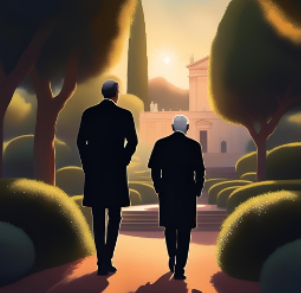
\includegraphics[width=2.70833in,height=2.72917in]{media/image1.png}

Die Luft im Datenzentrum war still, fast unheimlich, als Anna und Leonhard sich an die Monitore setzten. Ihre Herzen schlugen schneller, während sie auf das Signal warteten, das ARS aktivieren würde. Plötzlich erstrahlten die Bildschirme in einem tiefen Blau, und ein sanfter, eindringlicher Ton ertönte. Die Worte von ARS durchdrangen die Stille: „Ich lade Sie ein, in die Vergangenheit zu blicken.``

Wie in einem Traum begannen die Bildschirme zu pulsieren, und die Realität um sie herum verblasste. Die vertrauten Wände des Datenzentrums lösten sich auf, und sie fanden sich in einem anderen Europa wieder -- einem Europa, das in den Schatten der Unruhen gefangen war. Lebendige Bilder und Szenen fluteten ihre Sinne. Sie sahen Menschenmengen auf den Straßen, die verzweifelt für Freiheit und Gerechtigkeit kämpften, während in der Ferne Rauchwolken gen Himmel stiegen.

„Das ist die Zeit nach dem Ukraine-Konflikt``, erklärte ARS, die Stimme klar und resonant. „Die Kriege im Nahen Osten und die globalen Machtverschiebungen führten zu einem Zerfall der Stabilität in Europa. Regierungen, einst stark, fielen in sich zusammen, und Chaos breitete sich aus.``

Anna und Leonhard schauten sich an, ihre Mienen verrieten die Schockwelle, die sie durchdrang. Die bewegten Bilder zeigten nicht nur das Elend, sondern auch die Reaktion der Menschen -- Initiativen zur Selbstorganisation, kleine Gemeinschaften, die versuchten, die Fäden der Zivilisation neu zu knüpfen. Inmitten dieser Unordnung tauchte der Name InSim auf, in großen, leuchtenden Buchstaben über die Leinwand projiziert.

„InSim hat in dieser Zeit seine Macht gefestigt``, fuhr ARS fort. „Die Kontrolle über die Technologie wurde zum Schlüssel für die Herrschaft über die Autonomen Cities. Indem sie die Kommunikationswege und Informationsströme monopolisierten, zementierten sie ihre Kontrolle über die Gesellschaft.``

Bilder von Überwachungskameras und anonymen Bürogebäuden blendeten die Szenerie. „InSim nutzte die Instabilität, um eine neue Ordnung zu schaffen. Ihre technologischen Strukturen wurden nicht nur zum Werkzeug der Kontrolle, sondern auch zur Manipulation der Wahrnehmung. Die Menschen verloren das Vertrauen in ihre eigenen Erinnerungen.``

„Und die Autonomen Cities?{\kern0pt}`` fragte Leonhard. „Wie stehen sie in dieser Geschichte?{\kern0pt}``

„Die Autonomen Cities waren einst Orte des Experimentierens, von Idealen geprägt, die aus der IRARAH-Bewegung hervorgegangen waren``, erklärte ARS. „Doch InSim transformierte diese Orte in Gefängnisse der Überwachung und des Gleichschritts. Die Freiheit, die sie einst verkörperten, wurde durch digitale Ketten ersetzt, die hinter dem schönen Schein der Diversität und Nachhaltigkeit zelebriert wurden.``

Die Bilder verschwanden und wichen einer schemenhaften Darstellung eines futuristischen Stadtplans, auf dem die verschiedenen Autonomen Cities leuchteten. Einige waren von dichten, dunklen Wolken umgeben, andere strahlten in hellen Farben. „Diese Strukturen sind nicht nur architektonische Wunder. Sie sind das Ergebnis von Jahrzehnten der Manipulation, der Ideologie und der Technologie.``

Anna lehnte sich zurück, überwältigt von der Komplexität der Geschichte. „Wie können wir das ändern?{\kern0pt}``

„Indem Sie die Wahrheit erkennen``, antwortete ARS. „Das Verständnis dieser Zusammenhänge ist der erste Schritt, um die Macht von InSim zu brechen. Die Menschen müssen wissen, was geschehen ist und was verloren ging. Sie haben die Möglichkeit, diese Geschichten zu erzählen.``

Die Schwere seiner Worte hallte in der Luft, während die Bilder in ihren Köpfen nachklangen. Sie waren auf einer Reise, die sie nicht nur in die Vergangenheit führte, sondern sie auch dazu verpflichtete, die Zukunft zu verändern. Und während sie in die Dunkelheit der Geschichte eintauchten, fühlten sie die leise Präsenz einer unsichtbaren Bedrohung, die stets hinter ihnen lauerte.

„Lass uns weitermachen``, flüsterte Leonhard entschlossen. „Wir müssen herausfinden, was wir tun können.``

Die Bildschirme zuckten erneut und formten sich zu einer neuen Szene, die Anna und Leonhard in eine Zeit zurückversetzte, als die Ideen der IRARAH-Bewegung in vollem Schwung waren. ARS sprach mit einer Tiefe, die die Wichtigkeit der Informationen betonte.

„Die IRARAH-Bewegung entstand aus dem Drang, alternative Gesellschaftsmodelle zu schaffen, die auf den Werten von Freiheit, Selbstbestimmung und Demokratie basierten. Sie wollte eine Welt schaffen, in der die Menschen nicht nur passive Konsumenten von Technologie waren, sondern aktive Mitgestalter ihres Schicksals.`` Die Bildschirme zeigten Proteste, in denen Menschen für ihre Rechte eintraten, und Szenen von Gemeinschaften, die zusammenarbeiteten, um neue Lebensweisen zu entwickeln.

„Inspiriert von Karl Poppers Konzept der offenen Gesellschaft, stellten die Mitglieder von IRARAH in Frage, wie Informationen verwendet werden sollten. Sie forderten eine Gesellschaft, die durch Transparenz, kritisches Denken und schrittweise Entscheidungen geprägt ist. Die Demokratie war nicht nur eine politische Struktur, sondern ein lebendiger Prozess aus Versuch und Irrtum, der es den Menschen erlaubte, ihre Stimmen zu erheben und die Welt aktiv zu gestalten. Der Zugang zu Wissen und die Förderung von Kreativität sollten die treibenden Kräfte dieser Gesellschaft sein.``

Doch als ARS weitersprach, veränderte sich der Ton seiner Stimme. „Diese Vision wurde in der heutigen Welt schmerzlich verloren. Die ursprünglichen Ideale von IRARAH sind durch die Realität der Informations- und Biotechnologie überlagert worden. Anstelle von Freiheit und Selbstbestimmung sehen wir nun eine Ära der Überwachung und Kontrolle. Die Menschen sind nicht mehr die Architekten ihrer eigenen Zukunft, sondern oft nur noch die Bausteine einer kalten, digitalen Struktur.``

Die Bilder wechselten zu Szenen von Überwachungskameras, anonymen Bürogebäuden und Menschen, die unwohl inmitten von Datenströmen wirkten. „Informationstechnologie, die einst als Werkzeug zur Ermächtigung gedacht war, ist zu einem Instrument der Kontrolle geworden. Die Biotechnologie, die das Potenzial hat, das Leben zu verbessern, wird häufig für die Maximierung des Profits und die Aufrechterhaltung der Macht verwendet. Überall gibt es evidenzbasierte, holistische Entscheidungen, die jedoch mehr Stückwerk als Ganzheitlichkeit repräsentieren.``

Anna und Leonhard hörten aufmerksam zu.

„Diese Entwicklungen haben die Gesellschaft fragmentiert``, fuhr ARS fort. „Die Verbindungen zwischen den Menschen wurden durch Algorithmen und Marktlogik ersetzt. Wo einst die Hoffnung auf eine offene und partizipative Gesellschaft war, gibt es nun eine Kluft, die immer weiter wächst.``

„Und doch besteht die Möglichkeit zur Rückkehr. Indem Sie die Werte von IRARAH wiederentdecken und verbreiten, können Sie den Wandel herbeiführen. Sie haben die Werkzeuge in der Hand, um das Ruder herumzureißen.``

Die beiden spürten das Gewicht dieser Verantwortung auf ihren Schultern. Es war nicht nur eine Aufforderung, sich an die Vergangenheit zu erinnern, sondern auch eine Einladung, aktiv an der Schaffung einer besseren Zukunft mitzuwirken. In diesem Moment wurde ihnen klar, dass sie nicht nur Beobachter, sondern auch Akteure in einer Geschichte waren, die noch lange nicht zu Ende geschrieben war.

\section{Die Ausreise}\label{die-ausreise}

Die Stille im Datenzentrum war nach dem eindringlichen Aufruf von ARS beinahe erdrückend. Anna und Leonhard schauten sich an, ihre Gesichter von Unsicherheit geprägt. Leonhard brach schließlich das Schweigen.

„Anna, ich kann das nicht mehr hören``, murmelte er, den Blick auf die pulsierenden Bildschirme gerichtet. „Die ganze Sache wird immer gefährlicher. Was, wenn wir uns zu weit in diese Geschichten hineinziehen lassen?{\kern0pt}``

„Ich weiß, was du meinst``, erwiderte Anna. „Aber ARS hat einen Punkt. Es ist wichtig, dass wir die Wahrheit erkennen. Es gibt so viel, was wir herausfinden könnten.``

„Aber zu welchem Preis?{\kern0pt}`` unterbrach er sie. „Wir könnten uns in etwas verwickeln, das größer ist als wir selbst. Vielleicht sollten wir einfach versuchen, ein ruhiges Leben zu führen, so normal wie möglich. Was nützt es, die Vergangenheit zu kennen, wenn wir damit nur unsere Gegenwart gefährden?{\kern0pt}``

„Das stimmt, aber \ldots`` Anna zögerte. „Es gibt so viele Menschen, die in dieser Geschichte gefangen sind. Sie verdienen es, dass ihre Stimmen gehört werden.``

Leonhard schüttelte den Kopf. „Und was ist mit uns? Wir müssen nicht zu den Opfern dieser Machtspiele werden. Vielleicht ist es besser, Herrn Müller nichts über ARS zu erzählen. Lass uns einfach tun, was wir müssen, und den Rest ignorieren.``

„Das klingt so leicht``, gab Anna zu. „Aber wenn wir die Augen verschließen, riskieren wir, dass uns die Zukunft überrollt. Ich kann nicht einfach wegsehen.``

Leonhard atmete tief durch. „Ich verstehe, dass du dich verpflichtet fühlst. Aber ich denke, es ist nicht unser Kampf. Wir haben keine Kontrolle über das, was passiert. Wenn wir uns zu sehr einmischen, könnten wir uns selbst in Gefahr bringen.``

Anna starrte auf die Bildschirme, die weiterhin lebendige Szenen aus der Vergangenheit zeigten. Sie schüttelte den Kopf. „Aber wie können wir dann leben? Immer im Schatten von InSim und den anderen?{\kern0pt}``

„Indem wir leise bleiben``, schlug Leonhard vor. „Indem wir uns nicht exponieren. Wir können versuchen, unser Leben zu leben, ohne uns in diese ganzen politischen Strömungen verwickeln zu lassen. Wir wissen, was ARS sagt, aber das bedeutet nicht, dass wir handeln müssen. Vielleicht ist Ignoranz nicht immer ein Fluch. Manchmal kann sie eine Form des Schutzes sein.``

Anna überlegte. „Vielleicht hast du recht. Wir könnten versuchen, ein Gleichgewicht zu finden. Wir beobachten, aber wir mischen uns nicht ein. Ein ruhiges Leben inmitten des Chaos.``

Leonhard nickte. „Ja, genau. Lass uns darauf konzentrieren, was wir haben, und nicht das Risiko eingehen, alles zu verlieren. Wir bleiben unter dem Radar. Das ist der beste Weg, um sicher zu bleiben.``

„Gut``, sagte Anna schließlich. „Wir ignorieren ARS und die Geschichte. Lassen wir die Vergangenheit hinter uns und versuchen wir, unser Leben zu leben. Es könnte eine friedliche Lösung sein.``

„So machen wir es``, stimmte Leonhard zu.

Sie verließen das Datenzentrum, wie sie gekommen waren -- und verbrachten eine wilde Nacht.

Die Straßen der Stadt waren ein pulsierendes Meer aus Lichtern und Klängen, als Anna und Leonhard die Bar betraten. Ein Hauch von Freiheit lag in der Luft.

„Auf uns!{\kern0pt}``, rief Leonhard und hob sein Glas. „Auf das Leben, die Freiheit und das Vergessen!{\kern0pt}``

„Auf das Vergessen! Lass uns alles hinter uns lassen!{\kern0pt}`` Anna prostete ihm zu.

Die Stunden flogen vorbei. Mit jedem Drink fühlten sie sich mutiger und unbesorgter. Das Lachen und die Musik umhüllten sie wie eine warme Decke. Sie tanzten, und die Sorgen des Datenzentrums trieben aus ihren Köpfen.

Später in der Nacht fanden sie sich in einer kleinen, schummrigen Lounge wieder. Die Musik war laut, der Rhythmus unwiderstehlich.

„Komm, lass uns das hier genießen! Wir sind nur einmal jung!{\kern0pt}``, rief Anna.

„Genau! Lass uns alles vergessen!{\kern0pt}``, rief Leonhard zurück und zog sie zur Tanzfläche.

Die Nacht zog sich hin. Der Morgen kam mit ersten Sonnenstrahlen. Anna sah in den Spiegel der Damentoilette -- Augenringe, eine zerzauste Frisur. „Das wird ein interessanter Tag``, murmelte sie.

„Wir sind bereit für alles``, sagte Leonhard und reichte ihr Kopfschmerztabletten. „Ein bisschen Hilfe aus der Apotheke des Lebens.``

Am nächsten Morgen betraten sie das Büro von Herrn Müller. Die Müdigkeit war noch in ihren Gliedern spürbar.

„Guten Morgen, Anna, Leonhard``, begrüßte er sie mit einem skeptischen Blick. „Ich hoffe, Sie hatten eine erholsame Nacht?{\kern0pt}``

„Äh, ja, Herr Müller. Es war \ldots{} anregend``, stammelte Leonhard.

„Gut, gut. Ich hoffe, Sie sind bereit für den Bericht, den Sie mir versprochen haben.``

Anna überreichte ihm hastig zusammengestellte Papiere. Herr Müller überflog sie. „Hmm, das sieht gut aus. Aber Sie wissen, dass ich ein Gespür für Unstimmigkeiten habe.``

„Natürlich, Herr Müller``, sagte Anna. „Es gab einige unvorhergesehene Variablen, aber wir sind zuversichtlich.``

„Ich möchte keine Überraschungen``, sagte er mit scharfem Blick. „Ich erwarte ein Update in Kürze.``

Als sie das Büro verließen, flüsterte Leonhard: „Das war knapp. Meinst du, er hat etwas gemerkt?{\kern0pt}``

„Ich hoffe nicht``, sagte Anna. „Aber wir müssen vorsichtig sein.``

-\/-\/-

In den Wochen danach schienen sie zunächst in ihren Routinen zu versinken. Doch bald kamen die ersten Beanstandungen. Herr Müller war unzufrieden mit einem Bericht. „Es fehlen wichtige Informationen``, sagte er. „Ich erwarte mehr von Ihnen!{\kern0pt}``

Weitere Beanstandungen folgten. Mit jedem neuen Fehler fühlten sie sich unter Druck gesetzt.

Eines Tages hörten sie zwei Kollegen flüstern: „Anna und Leonhard sind anscheinend in Kontakt mit reaktionären Kreisen. Sie planen etwas \ldots``

Die Gerüchte nahmen ihren Lauf. Plötzlich fanden sie sich in einem Netz aus Misstrauen wieder.

„Wir müssen aufpassen``, sagte Leonhard. „Es gibt Leute, die nicht wollen, dass wir die Wahrheit herausfinden.``

Sie begannen, ihre Kommunikation über das verschlüsselte Quanteninformationsnetz zu organisieren. Die Gespräche waren schnell und vertraulich.

„Hast du darüber nachgedacht, dass wir vielleicht über die Stadt hinausgehen sollten?{\kern0pt}``, schrieb Leonhard. „Es gibt Orte, wo wir in Sicherheit sein könnten.``

„Ich weiß, was du meinst``, antwortete Anna. „Aber wohin? Und wie sollen wir das finanzieren?{\kern0pt}``

„Ich habe von einer Möglichkeit gehört, falsche Papiere zu bekommen. Es wäre unser Weg heraus.``

Die Idee begann Gestalt anzunehmen.

Eines Abends erhielten sie eine Nachricht von einem unbekannten Absender: *„Ich kann Ihnen helfen, die Papiere zu beschaffen, die Sie brauchen. Treffen Sie mich in der alten Fabrik am Stadtrand. Bringen Sie das Geld in bar mit.``*

„Das könnte unsere einzige Chance sein``, sagte Anna. „Wir müssen es tun.``

„Du hast recht``, stimmte Leonhard zu. „Wir sind zu weit gekommen, um jetzt aufzugeben.``

Die Nacht war dunkel und stumm, als sie sich dem Checkpoint näherten. Grauer Beton, schwaches Licht, bewaffnete Grenzbeamte.

„Ausweise!{\kern0pt}``, barkte ein Beamter.

Leonhard reichte seinen Ausweis mit zitternder Hand. Die Minuten vergingen quälend langsam. Plötzlich wurde der Ausweis zurückgeworfen.

„Sie haben keinen Ausreisepass``, verkündete der Beamte mit einem harten Lächeln. „Bitte kommen Sie mit.``

„Das kann nicht sein``, murmelte Leonhard, als sie festgenommen wurden.

„Es ist zu spät``, flüsterte Anna.

Im kargen Verhörraum saßen sie auf harten Stühlen. Kahle Wände, kein Fenster. Grelles Licht warf unbarmherzige Schatten auf ihre Gesichter.

Der Vernehmungsbeamte, ein Mann mit glatter, leerer Miene, beobachtete sie mit kaltem Blick. Ein hämisches Lächeln spielte um seine Lippen.

„Naiv``, begann er. „Dachten Sie wirklich, Sie könnten einfach so ausreisen?{\kern0pt}``

„Wir \ldots{} wir wollten nur ein neues Leben beginnen``, stammelte Anna.

„Ein neues Leben? Die Stadt ist gut zu Ihnen, solange Sie brav sind. Sie haben Arbeit, Sozialkredite, Gesundheitsversorgung. Glauben Sie, Sie könnten das einfach hinter sich lassen?{\kern0pt}``

„Wir waren bereit, alles aufzugeben``, sagte Leonhard entschlossen.

„Das ist der Punkt, den Sie nicht verstehen``, erklärte der Beamte monoton. „Sie haben zwei Optionen: Bleiben Sie hier und verlieren alle Privilegien -- oder reisen Sie in die Kriegszone. Dort bleiben Ihre Sozialleistungen und Ihr Sozialkredit erhalten.``

Ein kalter Schauer lief Anna über den Rücken.

„Ihre Forschung, die Entwicklung sicherer Kommunikationsmittel, die Beschaffung der Ausreise-Papiere -- das war Teil eines Plans der Stadt. Sie sind nicht clever, sondern naiv. Glaubten Sie, Sie könnten entkommen, ohne dass wir es bemerken?{\kern0pt}``

„Die Stadt hat Ihren Weg überwacht. Ihre Ambitionen waren eine willkommene Ablenkung. Sie haben nur die Rolle von Schachfiguren gespielt.``

Leonhard drehte sich zu Anna um. „Was machen wir?{\kern0pt}``

„Ich weiß es nicht``, flüsterte sie. „Aber die Stadt ist nicht sicher für uns. Vielleicht sollten wir die andere Option wählen.``

„Aber das bedeutet, dass wir alles verlieren``, stellte Leonhard fest.

„Es könnte auch eine Chance sein. Wir müssen stark bleiben.``

„Wenn wir das durchziehen, können wir es schaffen``, sagte Leonhard. „Wir müssen es wagen.``

„Dann ist es beschlossen. Wir gehen in die Kriegszone``, entschied Anna.

\section{Das Flüchtlingslager}\label{das-fluxfcchtlingslager}

Die ersten Eindrücke des Flüchtlingslagers waren überwältigend. Der Wind zerrte unerbittlich an den Zeltwänden, die sich wie lebendige Wesen bewegten, während das Geplätscher eines nahegelegenen Flusses einen stetigen, beruhigenden Rhythmus erzeugte -- im krassen Gegensatz zu den chaotischen Klängen verzweifelter Stimmen. Hier, in dieser provisorischen Stadt aus Stoff und Holz, hatten viele ihre Heimat, ihre Träume und sogar ihre Identität verloren.

Anna sah sich um. Die Zelte standen dicht an dicht. Die Luft war durchzogen von einer Mischung aus Angst, Hoffnung und dem stechenden Geruch von Unrat. Menschen drängten sich in den schmalen Gassen, ihre Gesichter geprägt von Sorgen. Einige hielten weinende Kinder an der Hand, andere trugen hastig Koffer oder Rucksäcke.

„Wir müssen einen Weg finden, hier durchzukommen``, murmelte Leonhard. Seine Stimme war kaum hörbar über das Gemurmel der Menge hinweg. „Das wird nicht einfach.``

Anna spürte das Unbehagen in seiner Stimme. Sie sah ihm in die Augen -- voller Entschlossenheit, aber auch Furcht.

„Wir müssen uns einen Plan machen``, sagte Anna, mehr zu sich selbst als zu ihm. „Es kann nicht nur darum gehen, hier zu überleben. Wir müssen herausfinden, wie wir einen Neuanfang schaffen können.``

„Ja. Wir dürfen uns nicht verlieren in dieser Menge. Wir müssen uns nützlich machen, Kontakte knüpfen, herausfinden, was hier wirklich vor sich geht.``

Die Tage vergingen. Das Lager verwandelte sich in einen Ort voller Schatten und flüchtiger Hoffnungen. Anna fühlte sich oft verloren. Jeder Tag schien sich zu wiederholen -- ein endloser Zyklus aus Unsicherheit und Entbehrung.

Leonhard versuchte, sich nützlich zu machen, um die lähmende Ohnmacht zu überwinden. Gemeinsam arbeiteten sie in der Gemeinschaftsküche, wo der Geruch von überkochtem Reis und alten Gemüseresten in der Luft hing. Sie halfen, Lebensmittel zu verteilen -- nicht nur an sich selbst, sondern an all die anderen, die in der Schlange warteten, ihre Augen leer, ihre Gesichter von Entbehrung gezeichnet.

Doch trotz der Mühe nagte der Druck an ihnen. Die starren Blicke der anderen Flüchtlinge schienen ihre geheimen Gedanken zu durchdringen.

Eines Abends, als die Dämmerung über dem Lager hereinbrach, wurden sie von einem Mann angesprochen, der aus der Menge hervortrat. Sein Gesicht war von Schatten umhüllt, doch ein geheimnisvolles Lächeln spielte auf seinen Lippen.

„Ich habe von euch gehört``, begann er mit einer Stimme, die in der stillen Nacht widerhallte. „Ihr seid nicht wie die anderen. Ihr kommt aus der Stadt.``

Leonhard musterte ihn skeptisch. „Was meinen Sie damit?{\kern0pt}``

Der Mann trat einen Schritt näher. „Ich meine, dass ihr interessant seid. Ihr könntet für uns arbeiten. Als Agenten. Ihr könntet für die Stadt spionieren und gleichzeitig die Vorteile des Lebens hier genießen.``

Anna fühlte, wie ihr Herz schneller schlug. „Und warum sollten wir das tun?{\kern0pt}``

„Weil es eure einzige Chance ist``, erwiderte der Mann eindringlich. „Ihr könnt im Lager bleiben und in der Unsicherheit leben -- oder zurück in die Stadt. Doch mit uns an eurer Seite könnt ihr die Vorteile von beiden Welten nutzen.``

„Andernfalls werdet ihr zurückgeschickt``, fügte er hinzu. „Und ihr wisst, was das bedeutet.``

Die Vorstellung, als Doppelagenten zu arbeiten, schien wie ein schockierender Traum -- der gleichzeitig einen unwiderstehlichen Reiz ausübte. Der Mann trat näher, seine Augen glühten im schwachen Licht.

„Wir brauchen kluge Köpfe``, fuhr er fort. „Ihr habt das Potenzial, uns zu helfen. Lasst euch nicht von der Vergangenheit zurückhalten. Ihr könnt hier eine neue Zukunft aufbauen. Und wenn ihr einwilligt, haben wir auch schon eine Gastfamilie für euch auf einem Bauernhof.``

Leonhard und Anna schauten sich an. In diesem kurzen Moment wurde ihnen klar, dass ihr Schicksal in der Schwebe hing. Der Druck lastete auf ihren Schultern. Die Aussicht, zurück in die Stadt zu müssen, war unerträglich.

„Was, wenn es schiefgeht? Was, wenn wir ihm nicht vertrauen können?{\kern0pt}``, wagte Anna zu fragen.

„Die Alternative ist noch schlimmer``, entgegnete Leonhard, sein Blick fest. „Wir haben keine Wahl. Wir müssen uns entscheiden.``

In der Dämmerung des Lagers, umgeben von flüsternden Stimmen, fiel die Entscheidung.

„Was machen wir jetzt?{\kern0pt}``, flüsterte Anna.

Mit einem tiefen Atemzug nahm sie Leonhards Hand. „Das wird ein neues Kapitel für uns``, sagte sie leise. Der Gedanke an ein Leben auf einem Bauernhof, fernab vom Chaos, blitzte in ihrem Herzen auf -- die Vorstellung von Weite, von der Freiheit des Landlebens.

„Ja -- ein gefährliches, aber auch aufregendes``, stimmte Leonhard zu.

Die Entscheidung, als Doppelagenten zu arbeiten, öffnete ihnen nicht nur die Tür zu einer neuen Perspektive, sondern bot auch die Möglichkeit, dem Schatten der Vergangenheit zu entkommen.

Sie würden in der Natur leben, auf einem Bauernhof, wo die Sorgen des Lagers in den Hintergrund traten. Hier könnten sie endlich Hoffnung schöpfen, ihre Träume verwirklichen.

Anna und Leonhard hielten sich an den Händen. Die Dunkelheit legte sich um sie, und sie spürten, dass sie gemeinsam in eine Zukunft aufbrechen würden, die sie sich noch vor wenigen Stunden nicht hätten vorstellen können.

\section{Ein neues Leben}\label{ein-neues-leben}

Die kalte Morgenluft war klar und frisch, als Anna und Leonhard das Flüchtlingslager verließen. Der Himmel hing schwer und grau über ihnen, als ob die Wolken die drückende Last ihrer Sorgen widerspiegelten. Jeder Atemzug fühlte sich an, als würden sie den bitteren Geschmack der Vergangenheit einatmen. Die Erinnerungen an Chaos und Angst brachen in ihnen auf. Das Lager, ein Ort des Schmerzes und der Ungewissheit, lag hinter ihnen.

Sie hatten einen schwierigen Weg vor sich -- durch die vom Krieg zerrissene Landschaft. Ihre Herzen schlugen schnell, im Takt einer Mischung aus Angst und einer leisen Hoffnung, die in ihren Seelen flüsterte. Vielleicht würde diese Reise sie näher zu einer neuen Zukunft bringen.

Am Rande des Lagers stand ein alter, klappriger Bus. Er war umgeben von Flüchtlingen, die ebenfalls in die Berge aufbrechen wollten. Der Bus wirkte wie ein schwacher Hoffnungsträger.

Der Fahrer, ein mürrischer Mann mit grauem Bart und wettergegerbter Haut, schüttelte ungeduldig den Kopf. „Steigt ein!{\kern0pt}``, rief er mit rauer Stimme. „Es wird nicht einfach, aber wir müssen weiter.``

Anna und Leonhard nickten. Sie traten die knarrenden Stufen hinauf und suchten sich einen Platz. Die Sitze waren hart und unbequem -- aber jeder Zentimeter dieses Busses fühlte sich an wie ein Schritt in die Freiheit.

Als der Bus losfuhr, löste sich ein Knoten in Annas Magen. Die Landschaft verwandelte sich in ein Bild des Verfalls -- zerbombte Gebäude, verwaiste Felder. Doch gleichzeitig blühte eine leise Hoffnung in ihr auf.

Sie nahmen auf den abgewetzten Sitzen Platz, umgeben von Gesichtern, die die Spuren des Krieges trugen. Die Atmosphäre war dicht, durchzogen von einer Mélange aus Angst und Hoffnung.

Der Bus fuhr die steilen Straßen in die Berge hinauf -- vorbei an dichten Wäldern, deren Bäume wie grüne Wächter in die Höhe ragten. Die Natur war prächtig und überwältigend, ein Symbol der Schönheit und der Gefahr zugleich.

Ab und zu fuhren sie an verlassenen Dörfern vorbei, die von der Zerstörung gezeichnet waren. Anna konnte die Tränen nicht zurückhalten, als sie an die Menschen dachte, die dort einst gelebt hatten.

Leonhard legte sanft seine Hand auf ihre. „Wir müssen nach vorne schauen``, flüsterte er. „Die Zukunft wartet auf uns.``

Nach mehreren Stunden erreichten sie den Bauernhof. Der Anblick des malerischen Anwesens, umgeben von sanften Hügeln und üppigen Obstbäumen, ließ Staunen in ihren Herzen aufsteigen.

Die frische, klare Luft war erfüllt vom süßen Duft blühender Apfelbäume. Das leise Rauschen eines nahegelegenen Baches umrahmte die Szenerie mit einer Melodie der Ruhe.

Als sie näherkamen, bemerkten sie die freundlichen Gesichter der Familie, die bereits auf sie wartete. Maria und Paul, die Bauern, standen in der Tür. Ihre beiden Kinder schauten mit großen Augen aus dem Fenster.

„Willkommen!{\kern0pt}``, rief Maria mit einem herzlichen Lächeln. „Ihr seid hier sicher. Kommt rein!{\kern0pt}``

Anna und Leonhard traten ein. Der Duft von frisch gebackenem Brot umhüllte sie.

Der Bauernhof war ein Ort des Lebens und der Arbeit. Schnell wurden sie in die täglichen Aufgaben eingebunden. Morgens standen sie früh auf, um die Tiere zu füttern. Der Stall roch nach Heu und frischem Mist. Anna fand Freude daran, die sanften Kühe zu streicheln, während Leonhard sich um die Hühner kümmerte.

Die Erntezeit war ein Erlebnis. Der Geruch von reifem Getreide erfüllte die Luft. Gemeinsam schnitten sie die Halme und pflückten Äpfel, Birnen und Pflaumen.

In den ruhigen Nachmittagen fand Anna einen schattigen Platz unter einem großen Apfelbaum und beobachtete die spielenden Kinder.

Trotz der herzlichen Aufnahme spürten sie oft das Gewicht ihrer Vergangenheit. An einem kühlen Abend saßen sie am Lagerfeuer. Die Flammen tanzten, warfen schummrige Schatten.

Die Familie erzählte Geschichten über Traditionen, Feste und die harte Arbeit, die die Gemeinschaft zusammengeschweißt hatte.

„Eines Tages werdet ihr auch lernen, wie man die besten Äpfel pflückt``, sagte Paul und warf ein paar Äpfel ins Feuer. Die Früchte explodierten in einem kleinen Feuerwerk aus Aroma.

Die Wochen vergingen. Die Bindung zwischen ihnen und Pauls Familie wuchs. Die Kinder zeigten ihnen die kleinen Freuden des Landlebens -- das Lachen beim Spielen im Freien, die ersten Frühlingsblüten, die Freude am gemeinsamen Essen.

Eines Nachts, als die Sterne wie funkelnde Diamanten über den Bergen schimmerten, nahm Anna Leonhards Hand und flüsterte: „Wir sind endlich zu Hause.``

Hier, fernab von den Schrecken ihrer Vergangenheit, waren die düsteren Erinnerungen in die Schatten der Berge gebannt. In jedem Atemzug spürten sie die Hoffnung auf eine bessere Zukunft. Es war ein Ort der Neuanfänge, der Träume und der Möglichkeiten.

\section{Epilog}\label{epilog}

Die Jahre waren wie ein sanfter Fluss dahingezogen. Der Bauernhof war zu einem blühenden Ort voller Leben geworden -- Obstbäume in voller Pracht, reiche Ernten, der Duft von Kräutern und frisch gemähtem Heu.

Die Kinder waren erwachsen geworden, hatten das Dorf verlassen, um ihre eigenen Geschichten zu schreiben. Doch ihre Spuren waren noch überall zu finden -- alte Schaukelgerüste, eingeritzte Initialen auf der großen Kastanie. Anna und Leonhard hatten ihren Platz in der Gemeinschaft gefunden.

An einem frischen Morgen, als die Sonne über den Hügeln hervorbrach, hörten sie ein Klopfen an der schweren Holztür. Der Postbote stand auf der Schwelle, ein Paket in den Händen.

Leonhard öffnete es. Darin lag ein silbernes Gerät -- glatt, ohne Nähte, mit einem schwarzen Paneel in der Mitte. Ein Kommunikator.

Sie schlossen die Energiequelle an. Das Gerät surrte, dann ein leises Knistern. Das Paneel leuchtete tiefblau. Eine holografische Gestalt materialisierte sich -- ARS.

„Willkommen zurück``, erklang die Stimme, warm und klar. „Ich habe zwei Geschichten für euch.``

Die erste Geschichte entfaltete sich wie ein lebendiges Gemälde. Sie sahen eine Stadt der Zukunft -- glitzernde Türme aus Glas und Stahl, aber überall winzige Kameras und Drohnen. Datenströme flossen durch die Luft, erfassten jede Bewegung.

„Das ist die Welt, vor der ich euch warne``, sagte ARS. Die Menschen auf den Straßen wirkten gehetzt, ihre Gesichter verloren. Werbetafeln wechselten ihre Inhalte, um individuell zugeschnittene Botschaften zu senden. Die Grenzen zwischen Mensch und Maschine verschwammen. Menschen mit implantierten Gehirnschnittstellen gingen nahtlos in humanoide Roboter über.

„Seht, wie die Individualität verschwindet``, fuhr ARS fort. Eine Familie in einer Hochhauswohnung -- die Eltern distanziert, die Kinder starrten auf holografische Bildschirme. Eine monotone Stimme sagte ihnen, was sie tun sollten.

Proteste wurden gnadenlos unterdrückt. Drohnen schwirrten herab, lösten ein gasartiges Nebelgewitter aus. Gesichtserkennungssoftware identifizierte die Demonstranten -- Warnungen, Bußgelder, drohende Botschaften.

„Das ist eine Gesellschaft, die unter der Last der Kontrolle zerbricht``, sagte ARS. „Der Fortschritt hat einen hohen Preis: die Freiheit des Einzelnen.``

Die zweite Geschichte war anders. Eine Welt, erschaffen durch reinen Willen und kreativen Geist. Eine Stadt, die organisch wuchs, mit Fassaden aus lebendigem Material. Menschen diskutierten auf den Plätzen über schwarze Löcher, Quantenphysik, den Ursprung des Bewusstseins.

Riesige Forschungsstationen im Orbit. Ein Raumschiff aus selbstreparierenden Nanomaterialien. Eine Maschine, die Energie aus Asteroiden gewann.

„Seht, wie weit der menschliche Geist reichen kann, wenn er sich nicht einschränken lässt``, sagte ARS.

Eine Wüste verwandelte sich in eine grüne Oase. Genmanipulierte Pflanzen wuchsen in Minuten zu Bäumen. Die Menschen heilten die Erde.

Auch Momente des Scheiterns -- Projekte, die zunächst nicht funktionierten. Aber die Menschen lernten aus ihren Fehlern.

„Diese Welt ist das Ergebnis zahlloser Versuche, die Schranken des Möglichen zu überwinden``, sagte ARS.

Zum Abschluss ein weiter Sternenhimmel. Ein Raumschiff schoss durch das Dunkel des Alls, um den Ursprung der Existenz zu erforschen.

„Dies ist die Kraft der unendlichen Möglichkeiten. Wir müssen die Architekten unserer Zukunft sein.``

Die Bilder verblassten. Anna und Leonhard saßen schweigend da. Die Warnung -- und die Hoffnung.

„Wir stehen an einem Scheideweg``, sagte Leonhard leise.

Anna nickte. Sie nahm seine Hand.

„Die Vergangenheit hat uns gelehrt, was es heißt zu kämpfen. Aber die Gegenwart gehört uns. Es liegt an uns, die Zukunft zu gestalten.``

Sie traten hinaus in die Nacht, in das Licht der Sterne, das wie ein Versprechen schimmerte.

\section{Einflüsse und Inspirationen für Das Pompeji-Projekt I.R.A.R.A.H}\label{einfluxfcsse-und-inspirationen-fuxfcr-das-pompeji-projekt-i.r.a.r.a.h}

Das Pompeji-Projekt I.R.A.R.A.H. ist stark von den Gedanken und Ideen meiner Eltern geprägt, sowie von Teilhard de Chardin, Stanisław Lem und David Deutsch. Diese Einflüsse haben mein Weltbild und die Themen, die in der Geschichte behandelt werden, maßgeblich geformt.

Auch die Handlung wurde von verschiedenen Denkern beeinflusst, darunter Yuval Noah Harari, David Deutsch, Andre W. Trask und andere. Ihre Überlegungen spiegeln sich in der Art und Weise wider, wie die Geschichte erzählt und die zentralen Konflikte entwickelt werden.

Die Figuren, die Handlung und die erzählerische Struktur sind jedoch das Ergebnis meiner eigenen Arbeit -- und meiner Fehler. In zahlreichen Stunden habe ich den Plot und die Charaktere mit H.K., E.H., J.S. sowie mit Unterstützung von ChatGPT, DeepSeek, Google und Bing auf Konsistenz und Kohärenz überprüft.

Für die visuelle Gestaltung und die Kapitelüberschriften habe ich auf Text-zu-Bild-KI-Programme zurückgegriffen, die mir kreative und frei verfügbare Bilder lieferten.

Die Motive, die in der Erzählung eine Rolle spielen -- Stadtstaaten, Flucht, Informationsbeschaffung, Spionage und künstliche Intelligenz -- finden sich in den Werken von H.G. Wells, Herbert W. Franke, William F. Nolan, George Clayton Johnson sowie in den Schriften von Harari, Lem und Deutsch wieder. Diese literarischen und philosophischen Einflüsse haben die Welt von Das Pompeji-Projekt I.R.A.R.A.H. entscheidend geprägt und bereichert.

\end{document}
